\documentclass[12pt]{article}

\usepackage{fontspec}
\setmainfont{TeX Gyre Pagella}

\usepackage{microtype}
\usepackage{geometry}
\geometry{margin=1in}

\usepackage{setspace}
\onehalfspacing

\usepackage{hyperref}
\usepackage{amsmath}
\usepackage{amssymb}
\usepackage{amsthm}

\usepackage{tikz}
\usetikzlibrary{arrows.meta, positioning, fit, shapes.geometric, calc, decorations.pathreplacing}
\usepackage{pgfplots}
\pgfplotsset{compat=1.18}

\usepackage{booktabs}
\usepackage{xcolor}
\usepackage{tcolorbox}
\tcbuselibrary{skins, breakable}
\usepackage{mdframed}

\theoremstyle{definition}
\newtheorem{definition}{Definition}[section]
\newtheorem{proposition}{Proposition}[section]
\newtheorem{remark}{Remark}[section]

\title{Interface Ecologies:\\
\large Motor Language, Process Invocation, and Computational Universality}
\author{Flyxion}
\date{\today}

\begin{document}

\maketitle

\begin{abstract}

Technical communities frequently engage in prolonged ideological
conflicts over programming languages, editors, keyboard layouts, and
development environments. These disputes are commonly framed as debates
about engineering correctness or computational capability. This essay
argues that such conflicts are better understood as ecological
phenomena emerging from what may be called \emph{interface ecologies}:
the interaction between human motor habits, cognitive metaphors, and
the symbolic grammars embedded within software tools.

Drawing on concepts from computability theory, particularly the
equivalence of the Turing machine and the lambda calculus
\cite{church1936,turing1936}, the paper observes that most modern
programming paradigms are computationally equivalent in expressive power.
Functional, imperative, object-oriented, and declarative systems
therefore differ primarily in their cognitive ergonomics rather than in
their theoretical capabilities \cite{backus1978}. Differences between
toolchains are best interpreted as alternative coordinate systems for
navigating the same computational space.

The analysis further examines how command-line environments, modal
editors, and compositional pipelines form a practical grammar of
process invocation that resembles algebraic function composition
\cite{fant2006,ritchie1974}. These interaction systems cultivate what
may be described as a \emph{motor language}, in which programming
actions become embodied sequences of symbolic transformations
\cite{norman1988}.

Within networked communities, however, such environments often generate
identity-forming cultural dynamics referred to here as the
\emph{scope memeplex}, wherein tools evolve from practical instruments
into ideological commitments. The resulting editor wars, keyboard wars,
and paradigm debates are interpreted not as technical necessities but
as sociotechnical phenomena produced by the alignment between human
cognition and particular interface grammars \cite{raymond2003}.

Recognizing the computational universality underlying these systems
suggests a modest conclusion: programming paradigms and toolchains are
best understood as dialects within a shared language of computation.
Their differences lie primarily in ergonomics, habit formation, and
cultural practice rather than in fundamental expressive power
\cite{kleene1952}.

\end{abstract}

\newpage
\tableofcontents
\newpage

\section{Introduction}

Technical culture is filled with arguments that appear, at first glance,
to be about engineering. Programmers debate editors, programming
languages, keyboard layouts, window managers, indentation styles,
frameworks, and operating systems with a degree of passion that often
exceeds the practical consequences of the tools themselves. These
conflicts frequently persist for decades, producing extensive bodies of
documentation, folklore, and rhetorical tradition.

Yet from the perspective of theoretical computer science, the intensity
of these debates is difficult to justify. The Church--Turing thesis
establishes that a wide range of formal computational models possess the
same expressive power \cite{turing1936,kleene1952}. Modern programming
paradigms, despite their surface differences, ultimately compile down to
machines capable of simulating one another. The computational substrate
remains stable even as programming languages and development environments
multiply.

If expressive power is largely equivalent across paradigms, then the
persistence of tooling wars must be explained elsewhere.

This essay proposes that many of these conflicts arise from what may be
called \emph{interface ecologies}: the interaction between human motor
habits, cognitive metaphors, and the symbolic grammars embedded in
software tools. Interfaces do not merely allow users to control
computers. They shape the ways in which programmers conceptualize
computation itself \cite{norman1988}. Over time, repeated interaction
with a particular environment produces stable cognitive and cultural
patterns. Commands become reflexes, keybindings become muscle memory,
and programming styles evolve to reflect the structures encouraged by
the tools in use.

Within such environments a phenomenon emerges that may be described as
the \emph{scope memeplex}. Technical tools gradually acquire ideological
significance. What begins as a practical choice becomes an identity,
and eventually a worldview. Editors become philosophies of text.
Programming languages become theories of computation. Keyboard layouts
become statements about efficiency, history, or aesthetic purity.

The resulting disputes often resemble intellectual conflicts, but they
are better understood as ecological competition between different
interaction grammars. Each toolchain creates a habitat in which certain
forms of reasoning feel natural and others appear awkward or
unintuitive \cite{brooks1975}.

The following sections examine these dynamics through a mixture of
historical reflection, theoretical analysis, and cultural observation.
Beginning with the well-known editor wars, the discussion traces how
interface design, motor cognition, and process composition interact to
produce distinct computational cultures. These cultures are then
considered in light of the deeper unity established by computability
theory \cite{church1936,turing1936}.

\begin{figure}[h]
\centering
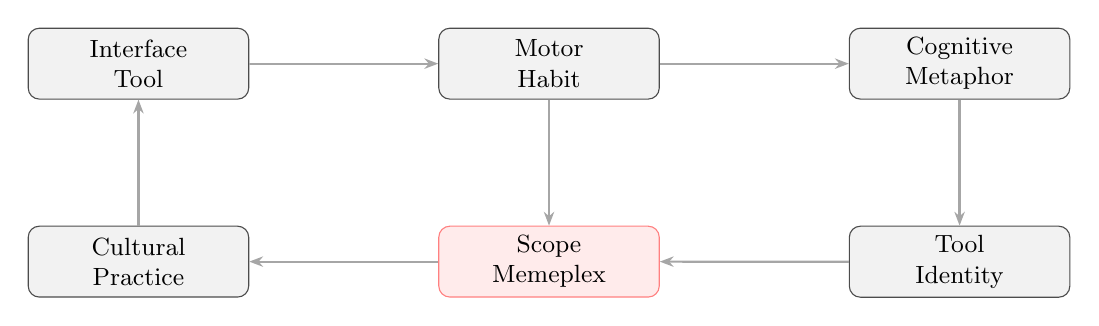
\begin{tikzpicture}[
  node distance=1.8cm,
  box/.style={rectangle, rounded corners=4pt, draw=black!70, fill=gray!10,
              minimum width=2.8cm, minimum height=0.9cm, font=\small, align=center},
  arrow/.style={-{Stealth[length=5pt]}, thick, gray!70}
]
  \node[box] (tool)    {Interface\\Tool};
  \node[box, right=2.4cm of tool] (motor)  {Motor\\Habit};
  \node[box, right=2.4cm of motor] (meta)  {Cognitive\\Metaphor};
  \node[box, below=1.6cm of meta] (ident)  {Tool\\Identity};
  \node[box, below=1.6cm of tool] (cult)   {Cultural\\Practice};
  \node[box, below=1.6cm of motor, fill=red!8, draw=red!50] (scope) {Scope\\Memeplex};

  \draw[arrow] (tool)  -- (motor);
  \draw[arrow] (motor) -- (meta);
  \draw[arrow] (meta)  -- (ident);
  \draw[arrow] (ident) -- (scope);
  \draw[arrow] (scope) -- (cult);
  \draw[arrow] (cult)  -- (tool);
  \draw[arrow] (motor) -- (scope);
\end{tikzpicture}
\caption{The interface ecology feedback loop. Repeated interaction with a
tool cultivates motor habit, which feeds into cognitive metaphor, which
hardens into tool identity, which cycles back through the scope memeplex
into cultural practice and tool selection.}
\label{fig:ecology_loop}
\end{figure}

Seen from this perspective, the great tooling wars of computing history
begin to resemble disputes between dialects spoken within a shared
language of computation.

The machines themselves remain remarkably indifferent.

\section{The Library of Lost Civilizations}

When I was younger I used to spend a great deal of time wandering through
computer labs and libraries, not because I needed to finish homework but
because I enjoyed watching small technological civilizations rise and
collapse in real time. Most people assume that the great ideological
conflicts of history are fought between nations, religions, or economic
systems. In reality many of the most bitter struggles have taken place
between programmers arguing about text editors at two o'clock in the
morning.

I remember the first time I encountered what historians now call the
Editor Wars. Two graduate students sat across from each other in front
of glowing CRT monitors, their faces illuminated by green text that
flickered like campfire light. One insisted that Emacs was not merely a
text editor but an entire computational universe in which every function
of life could eventually be implemented. The other claimed that Vim
represented the distilled essence of editing itself, a compositional
grammar of transformations whose elegance bordered on mathematical
inevitability.

Neither of them seemed aware that they were reenacting a drama as old as
civilization itself.

Their expressions reminded me of those sepia photographs from the
nineteenth century, the ones where soldiers stand stiffly beside rifles
almost as tall as they are. They looked like men who had seen too much
history and yet were still convinced that their particular hill was the
one worth dying on.

Except instead of rifles they were holding configuration files.

The tools in question, it should be noted, shared more than the combatants
acknowledged. Both Emacs and Vim represent stable points in a continuous
design space of interaction grammars, and both are Turing-complete
environments capable of hosting arbitrarily complex computation through
their extension mechanisms \cite{stallman2002,raymond2003}. Their
fundamental expressive power is equivalent. What differed was the
philosophy of access: one preferred a modal grammar of composable
transformations, the other a persistent, extensible runtime of Lisp
evaluation.

\section{The Scope Memeplex}

The truth about the editor wars is that they were never about editors.
They were manifestations of something far more powerful and far more
absurd, a phenomenon that scholars of digital anthropology now refer to
as the \emph{scope memeplex}.

\begin{definition}[Scope Memeplex]
A \emph{scope memeplex} is a self-reinforcing complex of tool preferences,
conceptual metaphors, social identity markers, and rhetorical traditions
that emerges within a technical community when the cognitive and motor
habits cultivated by a particular interface become inseparable from the
professional self-conception of its users.
\end{definition}

A scope memeplex emerges whenever a community of technically inclined
individuals begins to confuse a tool with a worldview. At first the tool
is merely practical. A programmer selects a keyboard layout, a shell
environment, or a development editor because it allows them to solve
problems efficiently. Over time the tool accumulates small rituals and
preferences. Keybindings are customized, configuration files are written,
shortcuts are memorized.

Eventually the tool ceases to be a tool and becomes an identity.

At that moment a transformation occurs. What was once a technical choice
becomes a moral position. The user no longer says that Vim works well
for them. They say that Vim is the \emph{correct} way to edit text. The
distinction may appear minor but the consequences are catastrophic.

For once correctness enters the conversation, disagreement becomes heresy.

\begin{figure}[h]
\centering
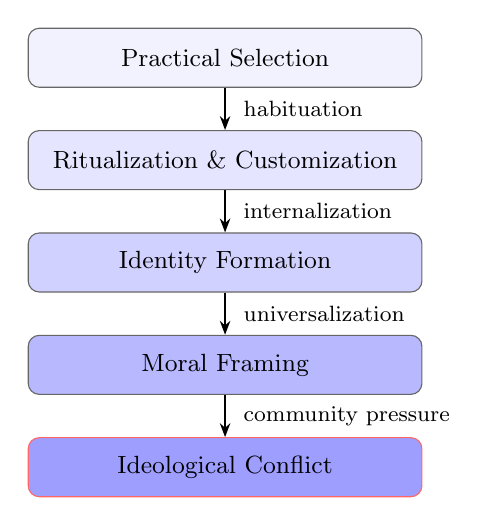
\begin{tikzpicture}[
  level/.style={rectangle, rounded corners, draw=black!60, fill=blue!#1,
                minimum width=5cm, minimum height=0.75cm, align=center,
                font=\small},
  arrow/.style={-{Stealth[length=5pt]}, thick}
]
  \node[level=5]  (p) at (0, 0)    {Practical Selection};
  \node[level=10] (r) at (0,-1.3)  {Ritualization \& Customization};
  \node[level=18] (i) at (0,-2.6)  {Identity Formation};
  \node[level=28] (m) at (0,-3.9)  {Moral Framing};
  \node[level=38, draw=red!60] (c) at (0,-5.2)  {Ideological Conflict};

  \draw[arrow] (p) -- (r) node[midway, right=3pt, font=\footnotesize] {habituation};
  \draw[arrow] (r) -- (i) node[midway, right=3pt, font=\footnotesize] {internalization};
  \draw[arrow] (i) -- (m) node[midway, right=3pt, font=\footnotesize] {universalization};
  \draw[arrow] (m) -- (c) node[midway, right=3pt, font=\footnotesize] {community pressure};
\end{tikzpicture}
\caption{The five-stage progression of the scope memeplex: from pragmatic
tool selection through habituation and identity formation to ideological
conflict. Each stage is driven by the preceding one, and the final stage
tends to obscure the contingency of the initial choice.}
\label{fig:memeplex_stages}
\end{figure}

Soon entire tribes begin to form around different conceptions of
computational virtue. One faction argues that software should be
infinitely extensible, a programmable cathedral in which every function
of life can be implemented through Lisp macros \cite{stallman2002}.
Another insists that software should be minimal, austere, a sharpened
blade of composable commands operating through modal grammar
\cite{mcilroy1978}. A third group believes that the entire debate is
irrelevant because modern integrated development environments provide
graphical tools that make the entire discussion obsolete.

Within a few years these positions harden into ideological camps.

Soon the mailing lists are burning.

\section{Civil War in the Terminal}

Historians often speak of the Browser Wars of the 1990s as though they
were an economic competition between corporations. This interpretation
is naïve. Corporations merely provided the artillery. The actual
combatants were millions of users who had unknowingly enlisted in a
conflict over the metaphysics of the web.

Internet Explorer loyalists believed that the browser should be
integrated into the operating system itself, an unavoidable
infrastructure layer upon which modern life would depend. Netscape
partisans imagined the browser as a portable gateway, an independent
interpreter of the open internet. Later generations would repeat the
same conflict under different banners, arguing about Chrome, Firefox,
and the eternal question of who truly owned the web.

But the pattern remained the same.

While the tribes fought each other with increasingly elaborate arguments
about standards compliance and rendering engines, the real victors
quietly sold advertisements against both sides.

This phenomenon is not unique to browsers. It appears everywhere
technological communities gather. The keyboard wars alone have produced
enough ideological literature to fill several libraries. QWERTY users
defend historical inertia with surprising passion \cite{yamada1980}.
Dvorak enthusiasts speak with the quiet conviction of reformers who
believe the world has taken a wrong turn somewhere around 1873. Colemak
users attempt a compromise that satisfies no one and therefore provokes
suspicion from everyone.

None of these groups realize that they are participating in a drama whose
outcome has already been decided.

Because while they debate finger travel distances and ergonomic purity,
the laptop manufacturers simply ship whatever layout the factories
already know how to produce.

\section{The Interface Wars}

Every generation of technologists believes that its conflicts are
fundamentally about technology. The browser wars, the editor wars, the
keyboard wars, the endless skirmishes over programming languages and
operating systems are typically narrated as engineering disputes.
Standards are invoked, performance benchmarks are cited, and carefully
measured latency graphs are deployed as though the outcome of these
debates could be determined by empirical fact alone.

Yet the emotional intensity of these conflicts tells a different story.

If the disputes were purely technical they would be settled quickly. A
superior design would emerge, the community would converge upon it, and
the matter would quietly close. Instead the arguments metastasize into
decades-long ideological struggles. Mailing lists burn with theological
certainty. Entire online cultures crystallize around configuration files.
Conferences fill with quiet factions who refuse to touch each other's
tools.

Such behavior cannot be explained by engineering considerations alone
\cite{brooks1975}.

The correct interpretation is ecological. What appears to be a debate
among engineers is in fact competition among symbolic organisms. Each
interface, language, or environment encodes a particular grammar of
action. Once adopted, that grammar restructures the cognitive and motor
routines of its host \cite{norman1988}. Commands become reflexes.
Keybindings become muscle memory. Patterns of thought begin to mirror
patterns of syntax.

At that point the interface is no longer merely a tool. It has become a
habitat.

Habitats compete.

The Vim user inhabits a world structured around modal grammar and
compositional transformation. Editing is conceived as algebra on text
streams. Motions combine with operators to form executable sentences
whose semantics are instantly realized within the buffer. To the
inhabitant of this ecosystem the arrow keys appear almost barbaric, an
inefficient relic of spatial navigation in a world where symbolic motion
should suffice.

The Emacs ecosystem evolves along a different trajectory. Here the editor
is not a grammar but an extensible organism. Lisp code permeates the
environment, allowing every function of the system to be rewritten from
within itself \cite{stallman2002}. The editor becomes a programmable
universe, a cathedral of recursion in which editing is merely one
activity among many.

Neither ecosystem is objectively correct. Both are stable evolutionary
niches.

Once established, however, each niche begins to defend its territory
with surprising ferocity. Tutorials become manifestos. Configuration
repositories become sacred texts. The technical language of documentation
gradually mutates into the rhetorical language of ideology.

What emerges is not a debate about tools but a civilizational narrative.

Each group begins to believe that its interface encodes the correct
philosophy of computing itself.

\section{The Spectacle of the Command Line}

It would be comforting to believe that the command line represents a
refuge from spectacle. After all, the terminal window appears austere
and monastic. Black background. Pale glyphs. A blinking cursor that
asks nothing except precision.

For decades its inhabitants have cultivated the belief that they live
outside the theater of technological fashion. While the graphical world
chases glossy interfaces and animated buttons, the command line community
imagines itself as a quiet order of ascetics who have renounced visual
decadence in favor of pure symbolic power \cite{raymond2003}.

Unfortunately this belief is only partially correct.

The terminal did not escape the spectacle. It merely produced a more
sophisticated version of it.

Within the command line ecosystem a peculiar aesthetic economy emerged.
Minimalism became a virtue signal. Configuration files grew into ornate
personal manifestos. Dotfile repositories appeared on public hosting
platforms, each presenting itself as the distilled wisdom of a
technological monk who had achieved enlightenment through careful
arrangement of keybindings and prompt colors.

Entire communities began to gather around the ceremonial sharing of
terminal screenshots.

One user would post an image of a meticulously arranged tiling window
manager, complete with translucent terminal panes and a prompt that
displayed the current Git branch, system load, weather forecast, and
the lunar phase of the current month. Another would respond with a
competing configuration that reduced the entire environment to a single
line of text and a blinking cursor, arguing that true enlightenment
required nothing more.

What began as an interface had become performance art.

The spectacle had simply moved from the graphical desktop to the symbolic
stage.

\section{Algorithmic Hegemony}

No ecosystem remains untouched by power for long. As digital culture
matured, new actors emerged whose influence extended beyond individual
interfaces and into the deeper structures of communication itself.

The modern programmer does not merely inhabit an editor or a shell. They
inhabit algorithmic infrastructure.

Discussion forums are filtered by recommendation engines. Documentation
is ranked by search algorithms. Social visibility is mediated by
engagement metrics that reward outrage, novelty, and tribal affirmation.
A developer who writes a careful explanation of a subtle technical issue
may receive modest attention, while another who posts a provocative
denunciation of some rival tool may attract thousands of responses
within hours.

The algorithms do not care which side wins the argument.

They only measure engagement.

Thus the ancient pattern repeats itself in a new technological
environment. Tribes form around symbols. Debates intensify. Entire
identities become fused with particular tools or languages. Meanwhile
the platforms hosting these conflicts quietly harvest the resulting
traffic, converting ideological energy into advertising revenue and
data analytics.

The spectacle has discovered automation.

\section{The Great Indentation Schism}

No study of technological sectarianism would be complete without
acknowledging the catastrophe that historians now refer to as the Great
Indentation Schism.

At first the disagreement seemed harmless. A small group of programmers
insisted that indentation should be represented by the tab character.
Another group argued that spaces produced more predictable alignment
across editors. Both sides presented technical arguments that, in
isolation, appeared reasonable.

But something strange occurred once the debate entered public discourse.

The indentation choice ceased to be a formatting preference and became
a statement of moral character. Tab advocates portrayed themselves as
defenders of semantic purity. Space advocates spoke of clarity,
discipline, and the sanctity of consistent formatting \cite{knuth1984}.
Entire style guides were written with the solemnity of constitutional
documents.

Soon automated tools appeared to enforce orthodoxy. Version control
systems began to flag violations. Continuous integration pipelines
rejected code that failed to conform to the chosen doctrine.

Repositories fractured.

Friendships dissolved.

At least one international conference reportedly included a hallway
altercation in which two engineers attempted to demonstrate the
superiority of their indentation method by drawing diagrams on a
whiteboard while security personnel looked on with visible confusion.

In retrospect it is difficult to determine exactly when the conflict
stopped being about whitespace.

Perhaps it never was.

\section{The Ideology of Tooling}

The final stage of any scope memeplex occurs when a community begins to
interpret its tools as expressions of philosophical truth. At this point
the interface no longer merely shapes behavior. It becomes a lens through
which reality itself is interpreted.

A developer who spends years working within a modal editor begins to
perceive the world as a sequence of composable transformations. Motions
and operators appear everywhere. Text streams resemble algebraic
structures awaiting manipulation.

Another developer immersed in graphical environments experiences
computing as spatial orchestration. Windows become containers of
activity. Menus represent hierarchical ontologies of action. The mouse
pointer becomes an extension of the hand itself \cite{norman1988}.

Each worldview feels natural to its inhabitant.

Each appears deeply strange to outsiders.

The tragedy is not that these perspectives differ. Diversity of
interaction models is one of the great strengths of computing culture.
The tragedy occurs when individuals mistake their personal habitat for
a universal law of nature.

At that moment the scope memeplex completes its life cycle.

A tool has become an ideology.

And somewhere, far above the battlefield of mailing lists and issue
trackers, the companies manufacturing keyboards and laptops continue
shipping the same hardware they always have, blissfully indifferent to
the metaphysical implications of the tab key.

\section{Motor Language and the Algebra of Interaction}

Most users imagine that computer interfaces are primarily visual systems.
Windows open, menus drop, icons glow politely in the corners of the
screen. Yet the deeper grammar of computing is not visual at all. It is
motor \cite{norman1988}.

Every interface trains the body. Keybindings become reflexes, shortcuts
become gestures, and gestures eventually become sentences spoken through
the hands. Over time a user develops what might be called a
\emph{motor language}: a repertoire of learned movements through which
intentions are translated into computational action.

\begin{definition}[Motor Language]
A \emph{motor language} is the system of learned, habituated motor
sequences through which a practitioner encodes computational intentions
as physical gestures. Motor language is interface-specific: each
toolchain cultivates a distinct vocabulary of motions, a grammar of
gesture sequences, and an implicit semantics that maps physical movements
onto symbolic transformations.
\end{definition}

In certain environments this motor language becomes surprisingly
sophisticated. Modal editors, compositional shells, and programmable
key layers transform the keyboard into something resembling an algebraic
instrument. Motions combine with operators. Commands compose with other
commands. A sequence of keystrokes ceases to be a simple instruction
and becomes instead a symbolic expression evaluated against the current
state of a text buffer or process stream.

\begin{figure}[h]
\centering
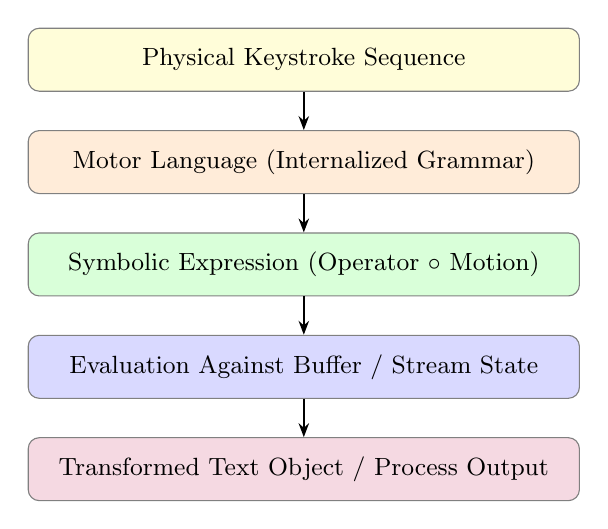
\begin{tikzpicture}[
  node distance=1.6cm,
  every node/.style={font=\small},
  layer/.style={rectangle, draw=black!50, rounded corners=4pt,
                minimum width=7cm, minimum height=0.8cm, align=center}
]
  \node[layer, fill=yellow!15] (phys)    at (0,0)   {Physical Keystroke Sequence};
  \node[layer, fill=orange!15] (motor)   at (0,-1.3){Motor Language (Internalized Grammar)};
  \node[layer, fill=green!15]  (sym)     at (0,-2.6){Symbolic Expression (Operator $\circ$ Motion)};
  \node[layer, fill=blue!15]   (eval)    at (0,-3.9){Evaluation Against Buffer / Stream State};
  \node[layer, fill=purple!15] (result)  at (0,-5.2){Transformed Text Object / Process Output};

  \foreach \a/\b in {phys/motor, motor/sym, sym/eval, eval/result}{
    \draw[-{Stealth[length=5pt]}, thick] (\a) -- (\b);
  }
\end{tikzpicture}
\caption{The motor language stack. A physical keystroke sequence is
interpreted through the practitioner's internalized motor grammar,
lifted to a symbolic expression combining operators and motions, evaluated
against the current editor or shell state, and realized as a transformed
output. Computational meaning emerges at the evaluation layer, not at
the physical layer.}
\label{fig:motor_stack}
\end{figure}

In this sense the interaction model of such systems begins to resemble
algebra more closely than navigation. One does not move a cursor so
much as apply transformations. A line becomes a structure. A paragraph
becomes an operand. Editing itself begins to feel less like typing and
more like manipulating symbolic forms within a constrained grammar of
operations.

To an outsider this behavior appears eccentric. To the practitioner it
feels inevitable.

\section{Keyboard Layouts as Cognitive Ecologies}

If motor language governs interaction, then the keyboard becomes its
geography. Each layout organizes the physical terrain through which the
fingers travel, and in doing so subtly shapes the rhythms of thought.

The persistence of the QWERTY layout is often explained through
historical inertia \cite{yamada1980}. A design created for mechanical
typewriters continues to dominate modern computing devices despite
repeated proposals for more efficient alternatives. Reformers
periodically arise to advocate layouts such as Dvorak or Colemak,
promising reduced finger travel and greater ergonomic harmony.

What these reform movements frequently underestimate is the ecological
stability of learned motor systems. Once a population has adapted to a
particular keyboard geography, the cost of migration becomes enormous.
Years of muscle memory must be dismantled and rebuilt. The fingers must
relearn their landscape.

\begin{figure}[h]
\centering
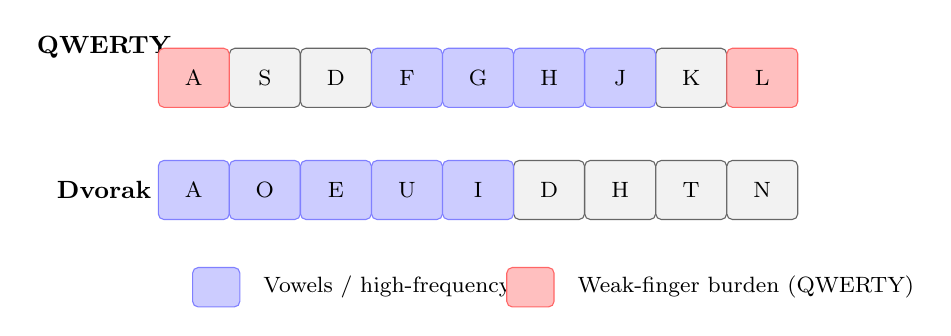
\begin{tikzpicture}[scale=0.95]
  \tikzset{key/.style={rectangle, draw=black!60, rounded corners=2pt,
                        minimum width=0.9cm, minimum height=0.75cm,
                        font=\footnotesize, fill=gray!10}}
  \tikzset{hlblue/.style={key, fill=blue!20, draw=blue!50}}
  \tikzset{hlred/.style={key, fill=red!25, draw=red!60}}

  % QWERTY home row label
  \node[font=\small\bfseries] at (-1.2, 0.4) {QWERTY};
  % Plain keys
  \foreach \letter/\x in {S/0.95,D/1.9,K/6.65}{
    \node[key] at (\x, 0) {\letter};
  }
  % Weak-finger keys (A, L)
  \node[hlred] at (0,   0) {A};
  \node[hlred] at (7.6, 0) {L};
  % High-frequency center (F G H J)
  \node[hlblue] at (2.85, 0) {F};
  \node[hlblue] at (3.8,  0) {G};
  \node[hlblue] at (4.75, 0) {H};
  \node[hlblue] at (5.7,  0) {J};

  % Dvorak home row label
  \node[font=\small\bfseries] at (-1.2, -1.5) {Dvorak};
  % Plain keys (consonants D H T N S)
  \foreach \letter/\x in {D/4.75,H/5.7,T/6.65,N/7.6}{
    \node[key] at (\x, -1.5) {\letter};
  }
  % Vowel-heavy home row (A O E U I)
  \node[hlblue] at (0,    -1.5) {A};
  \node[hlblue] at (0.95, -1.5) {O};
  \node[hlblue] at (1.9,  -1.5) {E};
  \node[hlblue] at (2.85, -1.5) {U};
  \node[hlblue] at (3.8,  -1.5) {I};

  % Legend
  \node[hlblue, minimum width=0.6cm, minimum height=0.5cm] at (0.3, -2.8) {};
  \node[font=\footnotesize, right] at (0.8, -2.8) {Vowels / high-frequency};
  \node[hlred, minimum width=0.6cm, minimum height=0.5cm] at (4.5, -2.8) {};
  \node[font=\footnotesize, right] at (5.0, -2.8) {Weak-finger burden (QWERTY)};
\end{tikzpicture}
\caption{Comparison of QWERTY and Dvorak home rows (simplified).
In Dvorak, vowels and the most common consonants of English are
concentrated on the home row, reducing finger travel; in QWERTY,
vowels are distributed across rows and weak fingers carry significant
load. The difference represents two incompatible cognitive ecologies
rather than a straightforwardly superior design \cite{yamada1980}.}
\label{fig:keyboard_compare}
\end{figure}

Thus keyboard layouts function less like tools and more like habitats.
Entire cognitive ecosystems evolve within their boundaries. Communities
of users emerge who share not only a physical layout but also a shared
motor culture: common shortcuts, shared typing rhythms, and an implicit
understanding of where meaning resides on the grid of keys.

Changing the layout therefore resembles ecological displacement. It is
not simply a matter of efficiency but of migration.

\section{The Terminal Monastic Tradition}

Within the broader culture of computing there exists a peculiar minority
who have chosen to inhabit the terminal almost exclusively. These
individuals speak of their environment with a mixture of pride and quiet
resignation, as though describing a remote mountain monastery that
outsiders would never fully understand.

The comparison is not entirely inappropriate.

The terminal demands a certain discipline. It offers little visual
guidance and few protective guardrails. Commands must be remembered
precisely. Mistakes are often immediate and unforgiving. Yet in
exchange for this austerity the terminal provides something rare in
modern computing: composability \cite{raymond2003,mcilroy1978}.

Small programs cooperate through simple textual interfaces. Output flows
into input. Commands form chains that resemble sentences written in a
minimal technical language. Over time the practitioner begins to perceive
these pipelines not merely as tools but as a method of reasoning.

The terminal thus cultivates a culture of quiet craftsmanship. Scripts
accumulate like marginal notes in a well-used notebook. Configuration
files become personal treatises on efficiency. The entire environment
evolves gradually, shaped by the long patience of someone who prefers
composition over spectacle.

It is perhaps the closest thing computing has to a monastic order.

\section{Algorithmic Hegemony and the Attention Economy}

Despite these pockets of quiet practice, no technical culture remains
isolated from the wider economic systems that surround it. In recent
decades the internet has introduced a new layer of influence that quietly
reshapes technological discourse.

Discussion platforms reward engagement rather than accuracy. Search
engines prioritize visibility rather than nuance. Recommendation
algorithms learn quickly that outrage travels farther than careful
explanation.

The result is a peculiar distortion of technical culture. Debates that
might once have remained small and localized now propagate across the
network with remarkable speed. Minor differences in tooling or workflow
are amplified into ideological conflicts. Entire communities organize
around symbolic distinctions that would previously have been considered
matters of personal preference.

In this environment the spectacle of technological debate becomes
self-sustaining. The arguments generate attention, the attention
generates revenue, and the revenue quietly reinforces the systems that
produced the argument in the first place.

No conspiracy is required. The infrastructure simply rewards noise.

\section{The Quiet Counterculture of Composable Systems}

Yet alongside the noise another tradition continues to persist. It does
not trend particularly well and rarely produces dramatic online debates.
Its practitioners are usually too busy building things to participate in
extended ideological arguments.

This tradition might be described as the counterculture of composability.

Its central belief is almost embarrassingly simple: software should
consist of small, understandable parts that cooperate through clear
interfaces \cite{mcilroy1978,raymond2003}. Instead of monumental
frameworks one constructs modest tools. Instead of monolithic systems
one builds chains of transformations. A problem becomes a sequence of
operations that can be reasoned about individually.

\begin{figure}[h]
\centering
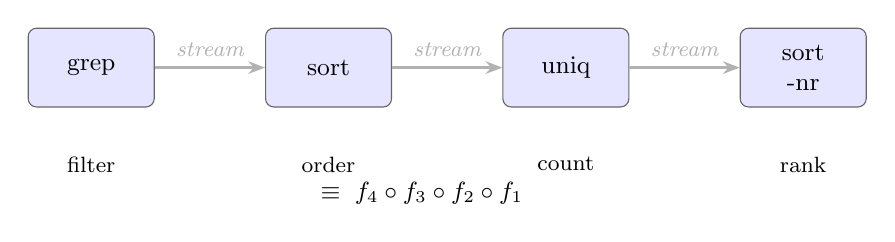
\begin{tikzpicture}[
  node distance=0.2cm,
  prog/.style={rectangle, draw=black!60, fill=blue!10, rounded corners=3pt,
               minimum height=1cm, minimum width=1.6cm, font=\small, align=center},
  pipe/.style={-{Stealth[length=6pt]}, very thick, gray!60},
  stream/.style={font=\footnotesize\itshape}
]
  \node[prog] (g)  {grep};
  \node[prog, right=1.4cm of g]  (s)  {sort};
  \node[prog, right=1.4cm of s]  (u)  {uniq};
  \node[prog, right=1.4cm of u]  (s2) {sort\\-nr};

  \draw[pipe] (g) -- node[above, stream]{stream} (s);
  \draw[pipe] (s) -- node[above, stream]{stream} (u);
  \draw[pipe] (u) -- node[above, stream]{stream} (s2);

  % Labels below
  \node[font=\footnotesize, below=0.5cm of g]  {filter};
  \node[font=\footnotesize, below=0.5cm of s]  {order};
  \node[font=\footnotesize, below=0.5cm of u]  {count};
  \node[font=\footnotesize, below=0.5cm of s2] {rank};

  % Math annotation
  \node[font=\small] at (4.2, -1.6) {$\equiv\; f_4 \circ f_3 \circ f_2 \circ f_1$};
\end{tikzpicture}
\caption{A Unix pipeline as function composition. Each process performs a
single transformation on a stream; the pipe operator connects them into
a composite function. The algebraic identity $f_4 \circ f_3 \circ f_2
\circ f_1$ captures the mathematical structure underlying what appears
to be a sequence of shell commands \cite{mcilroy1978,ritchie1974}.}
\label{fig:pipeline}
\end{figure}

Such work rarely produces dramatic demonstrations. It tends to look like
someone quietly writing scripts, refining keybindings, or improving a
pipeline that will save a few seconds each day. The improvements
accumulate slowly, almost invisibly, until the environment itself begins
to feel like an extension of thought.

From the outside this behavior appears mundane.

From the inside it feels like a kind of freedom.

\section{Escaping the Scope Memeplex}

If the scope memeplex represents the tendency of technical communities to
mistake tools for universal truths, then escaping it requires a small
but meaningful act of intellectual humility. One must recognize that
every interface is a local adaptation rather than a cosmic law.

Keyboard layouts provide an excellent illustration of this principle.

Consider the persistent fascination with the Dvorak layout. Advocates
describe it with the enthusiasm of reformers who have glimpsed an
alternate timeline in which typing evolved along a more rational
trajectory. The arrangement clusters vowels on the home row, distributes
common consonants across the strongest fingers, and minimizes the
acrobatic migrations required by the older QWERTY design \cite{yamada1980}.

To the initiated the experience can feel strangely peaceful. Words seem
to emerge from the keyboard with a fluid rhythm that resembles speech
more closely than mechanical tapping. Finger movement becomes smoother,
less frantic. One begins to suspect that the original keyboard designers
accidentally constructed a small obstacle course beneath the fingertips.

Yet the true lesson of Dvorak is not that it is universally superior.
Its real value lies in demonstrating that alternative motor ecologies
are possible at all. The keyboard need not remain frozen in the
industrial decisions of the nineteenth century.

A similar realization occurs when one moves beyond the confines of a
single language.

The Spanish keyboard introduces characters that expand the expressive
range of written communication. Accented vowels, the tilde of the
\~n, and the inverted punctuation of ¿ and ¡ remind the typist that
writing systems are shaped by the phonetic realities of human speech
rather than by the mechanical limitations of early typewriters.
Typing in Spanish therefore requires the fingers to acknowledge the
musical variation of language itself.

Arabic presents an even more profound shift in perspective. The script
flows from right to left, letters change form depending on their
position within a word, and the written line itself acquires a
calligraphic quality that resists the rigid geometry of Latin typography.
For a programmer accustomed to left-to-right syntax and rectangular
glyph grids, encountering Arabic text can feel like discovering that
writing is capable of motion.

The keyboard becomes not merely a tool for entering characters but a
gateway into another cognitive landscape.

What emerges from these encounters is a quiet but important insight.
Interfaces are cultural artifacts. They encode historical compromises,
linguistic assumptions, and ergonomic guesses made by designers who
rarely imagined the full diversity of their future users \cite{norman1988}.

Recognizing this fact dissolves much of the ideological fervor
surrounding technological tools. The keyboard wars, the editor wars,
the endless debates over the correct arrangement of symbols begin to
appear less like battles for truth and more like the natural turbulence
of overlapping design traditions.

Escaping the scope memeplex therefore does not require the abandonment
of one's preferred tools. It simply requires remembering that they are
preferences rather than commandments.

A Vim user may continue to compose elegant modal sentences. An Emacs
devotee may continue to extend their programmable universe. A Dvorak
typist may enjoy the gentle choreography of balanced finger motion while
a QWERTY typist proceeds perfectly content with inherited muscle memory.

The difference is subtle but significant.

Once the illusion of universality fades, the tools return to their
proper role. They become instruments rather than identities.

And in that moment the long wars of configuration begin to look less
like ideological struggles and more like what they always were: small
disagreements about how best to arrange one's hands on a piece of
plastic.

\section{Computational Universality and the Limits of Paradigm Wars}

Many of the ideological conflicts surrounding programming languages and
development environments are implicitly grounded in the belief that
different paradigms represent fundamentally different kinds of
computational power. Advocates of functional programming frequently
describe their methods as mathematically pure, while proponents of
imperative systems emphasize control over state and machine behavior
\cite{backus1978}. Object-oriented systems promise modular abstraction,
while logic programming communities emphasize declarative reasoning.

Yet from the perspective of theoretical computer science, these disputes
often obscure a deeper unity.

The foundational result underlying modern computation is the equivalence
between multiple formal models of computation developed during the
1930s. Two of the most influential are the Turing machine, introduced
by Alan Turing, and the lambda calculus, introduced by Alonzo Church
\cite{church1936,turing1936}. Despite their radically different
formulations, both systems were shown to characterize the same class
of computable functions \cite{kleene1952}.

\subsection{Turing Machines}

A Turing machine is defined as a tuple
\[
M = (Q, \Sigma, \Gamma, \delta, q_0, q_{accept}, q_{reject})
\]
where $Q$ is a finite set of states, $\Sigma$ is the input alphabet,
$\Gamma$ is the tape alphabet with $\Sigma \subseteq \Gamma$, and
$\delta$ is a transition function
\[
\delta : Q \times \Gamma \rightarrow Q \times \Gamma \times \{L,R\}.
\]

The machine operates by reading and writing symbols on an unbounded tape
while moving a read--write head left or right \cite{turing1936}. Although
this model appears mechanically primitive, it has been proven capable of
simulating any algorithm that can be described by effective procedures.

\begin{figure}[h]
\centering
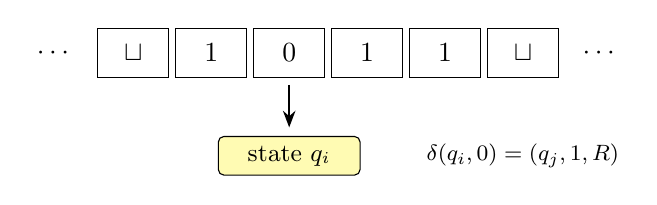
\begin{tikzpicture}[scale=0.9]
  % Tape cells
  \foreach \i/\c in {0/$\sqcup$,1/1,2/0,3/1,4/1,5/$\sqcup$}{
    \draw (\i*1.1, 0) rectangle (\i*1.1+1, 0.7);
    \node at (\i*1.1+0.5, 0.35) {\c};
  }
  % Ellipses
  \node at (-0.6, 0.35) {$\cdots$};
  \node at (6.6+0.5, 0.35) {$\cdots$};

  % Read-write head
  \draw[-{Stealth[length=6pt]}, thick] (2*1.1+0.5, -0.1) -- (2*1.1+0.5, -0.7);
  \node[rectangle, draw=black, fill=yellow!30, rounded corners=2pt,
        font=\small, align=center, minimum width=1.8cm] at (2*1.1+0.5,-1.1) {state $q_i$};

  % Transition annotation
  \node[font=\footnotesize, right] at (4.5, -1.1)
        {$\delta(q_i, 0) = (q_j, 1, R)$};
\end{tikzpicture}
\caption{A Turing machine reading cell 2 (symbol 0) in state $q_i$.
The transition function $\delta$ specifies the new state $q_j$, the
symbol written (1), and the head direction (R). The unbounded tape
provides the machine's working memory \cite{turing1936}.}
\label{fig:turing}
\end{figure}

\subsection{Lambda Calculus}

The lambda calculus, by contrast, is an abstract system of symbolic
function manipulation \cite{church1936}. Its syntax is built from three
simple constructs:
\[
e \;::=\; x \;\mid\; (\lambda x.\, e) \;\mid\; (e_1 \; e_2)
\]
where $x$ represents variables, $\lambda x.e$ represents function
abstraction, and $(e_1 \; e_2)$ represents function application.

Computation occurs through the rule of $\beta$-reduction:
\[
(\lambda x.\, M)\; N \;\longrightarrow_\beta\; M[x := N].
\]

Despite its minimal syntax, the lambda calculus is capable of expressing
arbitrary recursive functions through appropriate encodings. For
instance, the Church numeral $\mathbf{n}$ encodes the natural number
$n$ as the $n$-fold application of a function $f$ to an argument $x$:
\[
\mathbf{n} \;=\; \lambda f.\, \lambda x.\, f^n\, x.
\]

\begin{figure}[h]
\centering
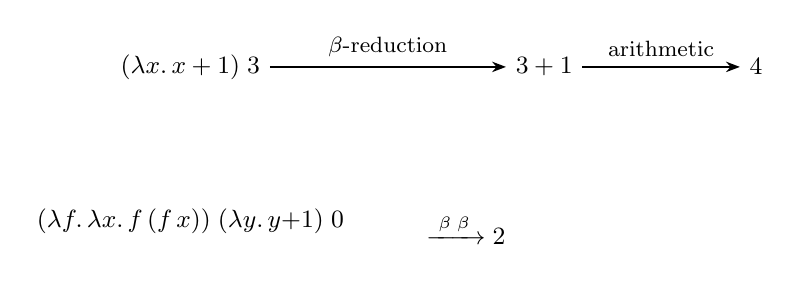
\begin{tikzpicture}[
  node distance=1.4cm,
  term/.style={font=\small},
  arrow/.style={-{Stealth[length=5pt]}, thick}
]
  \node[term] (A) {$(\lambda x.\, x + 1)\; 3$};
  \node[term, right=3cm of A] (B) {$3 + 1$};
  \node[term, right=2cm of B] (C) {$4$};

  \draw[arrow] (A) -- node[above, font=\footnotesize]{$\beta$-reduction} (B);
  \draw[arrow] (B) -- node[above, font=\footnotesize]{arithmetic} (C);

  \node[term, below=1.4cm of A] (D)
    {$(\lambda f.\,\lambda x.\, f\,(f\, x))\;(\lambda y.\, y{+}1)\; 0$};
  \node[term, right=0.8cm of D, yshift=-0.1cm, font=\small] (E)
    {$\xrightarrow{\;\beta\;\beta\;} 2$};
\end{tikzpicture}
\caption{Beta-reduction in the lambda calculus \cite{church1936}. The
upper row shows a simple application; the lower row shows Church numeral
2 evaluated against the successor function and zero, yielding~2.}
\label{fig:lambda}
\end{figure}

\subsection{Equivalence and the Church--Turing Thesis}

The key theoretical result is that these two models are computationally
equivalent \cite{kleene1952}. Every lambda calculus expression can be
simulated by a Turing machine, and conversely, the behavior of any
Turing machine can be represented within the lambda calculus.

\begin{proposition}
\label{prop:equiv}
The class of functions computable by Turing machines equals the class
of functions expressible in the untyped lambda calculus, and both equal
the class of general recursive functions.
\end{proposition}

This equivalence forms the conceptual basis of the Church--Turing thesis,
which informally states that any effectively computable function can be
computed by a Turing machine, or equivalently by any other sufficiently
expressive computational formalism \cite{kleene1952}.

\begin{figure}[h]
\centering
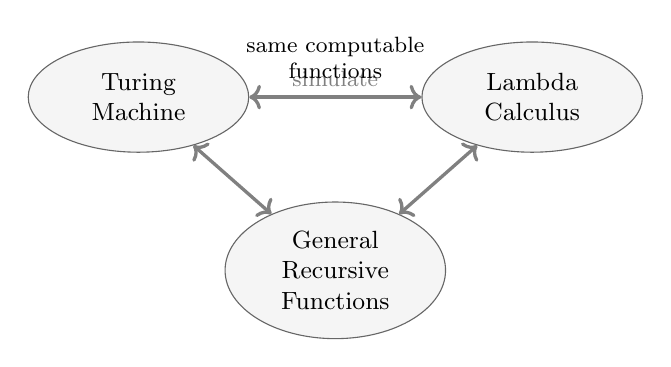
\begin{tikzpicture}[
  oval/.style={ellipse, draw=black!60, minimum width=2.8cm,
               minimum height=1.4cm, font=\small, align=center,
               fill=gray!8},
  barrow/.style={<->, very thick, gray}
]
  \node[oval] (TM)  at (-2.5, 0)  {Turing\\Machine};
  \node[oval] (LC)  at (2.5, 0)   {Lambda\\Calculus};
  \node[oval] (GR)  at (0, -2.2)  {General\\Recursive\\Functions};

  \draw[barrow] (TM) -- node[above, font=\footnotesize]{simulate} (LC);
  \draw[barrow] (TM) -- (GR);
  \draw[barrow] (LC) -- (GR);

  \node[font=\footnotesize, align=center] at (0, 0.5)
    {same computable\\functions};
\end{tikzpicture}
\caption{The equivalence triangle of computation \cite{kleene1952}.
Turing machines, lambda calculus, and general recursive functions all
define the same class of computable functions. Each can simulate the
others, so no paradigm built on any of these foundations possesses
strictly greater expressive power.}
\label{fig:equiv_triangle}
\end{figure}

\subsection{Consequences for Programming Paradigms}

Once this equivalence is recognized, the ideological disputes between
programming paradigms appear in a new light. Imperative languages,
functional languages, logic programming systems, and object-oriented
frameworks all compile down to computational mechanisms that are
ultimately equivalent in expressive power \cite{backus1978}.

Differences among them therefore arise primarily from factors such as
ergonomics, cognitive models, abstraction mechanisms, and historical
development rather than from fundamental computational capability.

\begin{table}[h]
\centering
\small
\begin{tabular}{lllll}
\toprule
\textbf{Paradigm} & \textbf{Primary Model} & \textbf{State} &
  \textbf{Primary Metaphor} & \textbf{Universal?} \\
\midrule
Imperative       & State machine       & Explicit mutable & Commands          & Yes \\
Functional       & Lambda calculus     & Implicit/managed & Expressions       & Yes \\
Object-oriented  & Message passing     & Encapsulated     & Objects           & Yes \\
Logic            & Resolution proof    & Constraint store & Relations         & Yes \\
Dataflow         & Signal graph        & Stream-based     & Pipelines         & Yes \\
\bottomrule
\end{tabular}
\caption{Five major programming paradigms and their relationship to
computational universality. Despite dramatic differences in primary
metaphor and state management strategy, all are computationally
universal: each can simulate any of the others, given sufficient
resources. The conflicts between their communities must therefore be
understood as ergonomic and cultural rather than fundamental
\cite{backus1978,kleene1952}.}
\label{tab:paradigms}
\end{table}

A functional language may represent computation through the evaluation
of expressions, while an imperative language may describe state
transformations step by step. Yet both can simulate the other. A
functional program can encode mutable state through monads or explicit
state passing, while an imperative system can simulate higher-order
functions through closures or equivalent constructs.

In theoretical terms, they occupy different regions of the same
computational landscape.

\subsection{Implications for the Scope Memeplex}

This observation returns us to the broader argument of the essay. The
intensity of programming paradigm wars cannot be explained by genuine
differences in expressive power, since such differences do not exist at
the level of computability theory \cite{kleene1952}.

Instead the conflicts arise from the interaction between human cognitive
preferences and the environments in which those preferences are
cultivated. Developers internalize particular interaction grammars and
conceptual metaphors through repeated practice \cite{norman1988}. Over
time those habits become intertwined with professional identity.

What begins as a practical preference gradually transforms into a
philosophical commitment.

From the standpoint of theoretical computation, however, these disputes
resemble arguments over dialects spoken within the same language.
Different paradigms provide alternative syntactic pathways through the
same space of computable functions.

The machines beneath them remain quietly indifferent.

\section{Composability, Pipelines, and the Practical Lambda}

While the theoretical equivalence between the Turing machine and the
lambda calculus demonstrates that all sufficiently expressive
programming paradigms share the same computational power, it does not
imply that all paradigms are equally pleasant for human beings to use.
The question therefore shifts from expressive capability to cognitive
ergonomics.

Certain programming environments appear to resonate particularly well
with the algebraic intuitions that underlie the lambda calculus. The
classical Unix toolchain provides one of the clearest examples
\cite{ritchie1974,mcilroy1978}.

In the Unix philosophy, programs are intentionally small and narrowly
focused \cite{raymond2003}. Each tool performs a single transformation
on a stream of textual data. The output of one program can be directed
into the input of another through the pipe operator. Over time,
programmers develop the habit of constructing chains of transformations
that resemble the composition of mathematical functions.

A simple pipeline illustrates the pattern:
\[
\texttt{grep pattern file | sort | uniq -c | sort -nr}
\]

Although written as a shell command, the structure mirrors the
composition of functions in mathematics. If we interpret each command as
a transformation on a stream $S$, the pipeline corresponds conceptually
to
\[
f_4(f_3(f_2(f_1(S)))).
\]

The pipe operator therefore behaves as a practical syntax for function
composition. What appears to be a sequence of shell commands is
effectively an executable expression describing how data flows through
a series of transformations \cite{fant2006}.

This compositional style echoes the operational semantics of the lambda
calculus. In both systems, complex behavior emerges through the repeated
application and composition of small functions. The programmer does not
explicitly describe every intermediate state of the system. Instead they
construct a chain of transformations whose evaluation produces the
desired result.

\subsection{Modal Editing and Symbolic Transformation}

A similar structure appears in modal text editors such as Vim. Commands
within such editors often take the form of composable expressions in
which operators combine with motions to produce transformations of the
text buffer.

For example, the command
\[
\texttt{d3w}
\]
may be interpreted as an operator $d$ (delete) applied to the motion
$3w$ (three words). The resulting expression performs a transformation
on the text object currently in focus.

More generally, the modal editing grammar follows the pattern:
\[
[\text{count}]\;\text{operator}\;[\text{count}]\;\text{motion}
\]
where the operator specifies the type of transformation ($d$: delete,
$c$: change, $y$: yank, $>$: indent) and the motion specifies the text
object (word, sentence, paragraph, matching delimiter, line, \ldots).
The composition of these elements produces a small but expressive
algebra of text transformations.

\begin{figure}[h]
\centering
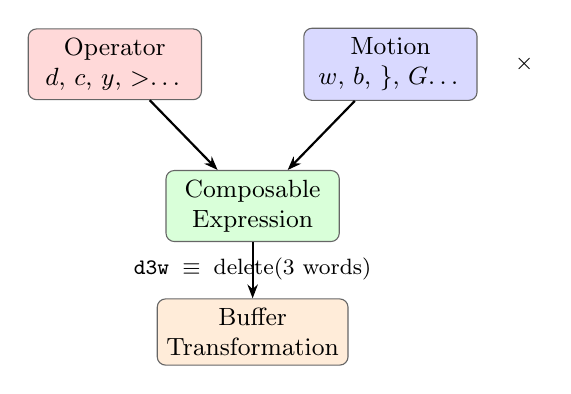
\begin{tikzpicture}[
  box/.style={rectangle, draw=black!60, rounded corners=3pt,
              minimum width=2.2cm, minimum height=0.8cm, align=center,
              font=\small},
  arrow/.style={-{Stealth[length=5pt]}, thick}
]
  \node[box, fill=red!15]    (op)  at (0,0)   {Operator\\$d$, $c$, $y$, $>$\ldots};
  \node[box, fill=blue!15]   (mo)  at (3.5,0) {Motion\\$w$, $b$, $\}$, $G$\ldots};
  \node[box, fill=green!15]  (ex)  at (1.75,-1.8) {Composable\\Expression};
  \node[box, fill=orange!15] (buf) at (1.75,-3.4) {Buffer\\Transformation};

  \draw[arrow] (op) -- (ex);
  \draw[arrow] (mo) -- (ex);
  \draw[arrow] (ex) -- (buf);

  \node[font=\footnotesize] at (5.2, 0) {$\times$};
  \node[font=\footnotesize] at (1.75, -2.6)
        {$\texttt{d3w} \;\equiv\; \text{delete}(\text{3 words})$};
\end{tikzpicture}
\caption{The compositional grammar of modal text editing. An operator
and a motion combine to form a composable expression that is evaluated
against the current buffer state, producing a transformation. The
resulting algebra constitutes a domain-specific language for symbolic
text manipulation.}
\label{fig:modal_grammar}
\end{figure}

In this sense modal editing begins to resemble a small domain-specific
language for symbolic manipulation. Text is not merely typed or erased;
it is transformed through composable operations whose syntax becomes
internalized through motor memory.

The user's hands effectively speak a compact grammar of transformations.

\subsection{Motor Cognition and Functional Composition}

The convergence between these interaction models and formal computation
theory may explain why certain programmers experience command-line
environments as unusually expressive. When pipelines, modal commands,
and scripting languages are combined, the entire system begins to feel
less like a graphical workspace and more like an algebraic instrument.

Problems are decomposed into transformations.
Transformations are composed into pipelines.
Pipelines become scripts.
Scripts evolve into systems.

In effect, the programmer constructs executable mathematics \cite{knuth1984}.

\subsection{The Dissolution of Paradigm Absolutism}

Recognizing this relationship does not imply that one interface or
paradigm is objectively superior. The equivalence results of theoretical
computer science remind us that all sufficiently expressive systems can
ultimately simulate each other \cite{kleene1952}. What differs is the
cognitive path by which the programmer arrives at the solution.

Some environments emphasize spatial reasoning and visual organization.
Others emphasize symbolic manipulation and functional composition.
Still others prioritize declarative specification or object
encapsulation.

Each represents a different navigational strategy through the same
computational universe.

The ideological intensity of programming paradigm wars therefore
reflects not genuine differences in expressive power but the deep
psychological attachment that develops when a particular interface
aligns with a programmer's preferred mode of thought.

From the standpoint of computability theory, however, these conflicts
resemble arguments over different coordinate systems used to describe
the same mathematical space.

The machine beneath them continues to evaluate functions with serene
indifference.

\section{Process Invocation as a Language}

The command line environment is often described as an interface. From a
computational perspective, however, it may be more accurately understood
as a language for invoking and composing processes \cite{fant2006}. In
this view the shell does not merely execute programs but provides a
grammar through which processes are orchestrated into larger
computational structures.

A shell command is therefore not simply an instruction but a sentence in
a process invocation language.

\begin{definition}[Process Invocation Language]
A \emph{process invocation language} is a formal grammar whose primitive
symbols denote executable processes and whose composition operators
describe the communication topology, data flow, and scheduling
constraints that govern their interaction. The shell constitutes the
canonical example: its primitives are Unix programs, its composition
operators are the pipe (\texttt{|}), redirection (\texttt{>},
\texttt{<}), and job control operators, and its semantics are defined
by the operating system's process model \cite{ritchie1974}.
\end{definition}

The primitive elements of this language correspond to executable
programs. Each program accepts input, performs a transformation, and
produces output \cite{mcilroy1978}. The shell provides syntactic
operators that describe how these transformations are composed,
redirected, or executed in parallel. Pipes connect the output of one
process to the input of another, redirection operators bind streams to
files, and control constructs allow the user to specify conditional
execution or iterative behavior.

This structure gives rise to a distinctive computational idiom. Rather
than writing large monolithic programs, users construct pipelines of
small cooperating processes. A typical command might appear as
\[
\texttt{cat data.txt | grep pattern | sort | uniq -c | sort -nr}
\]

Each stage in the pipeline performs a simple transformation on the data
stream \cite{raymond2003}. The pipe operator expresses the composition
of these transformations, producing behavior that emerges from the
interaction of multiple small components.

Conceptually this resembles function composition in mathematics. If
each program is interpreted as a function on a stream $S$, then the
pipeline above corresponds to a composition
\[
f_5(f_4(f_3(f_2(f_1(S))))).
\]

The shell thus acts as a lightweight calculus of processes.

\subsection{Invocation Semantics and Operating System Architecture}

From an operating systems perspective, each command within a pipeline
corresponds to a process invocation \cite{ritchie1974}. The shell
performs a sequence of system calls that create new processes, establish
communication channels between them, and schedule their execution. Pipes
are implemented as kernel-managed buffers that connect the standard
output of one process to the standard input of the next.

\begin{figure}[h]
\centering
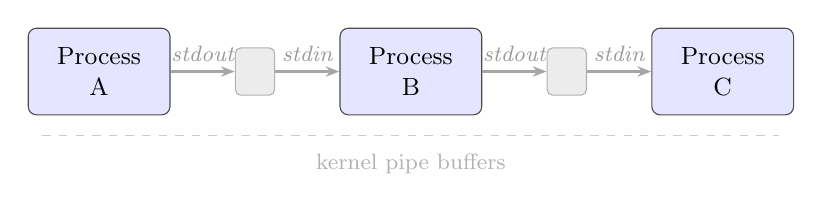
\begin{tikzpicture}[scale=0.9,
  proc/.style={rectangle, draw=black!70, fill=blue!10, rounded corners=3pt,
               minimum width=1.8cm, minimum height=1.1cm, font=\small, align=center},
  pipe/.style={rectangle, draw=gray!60, fill=gray!15, rounded corners=2pt,
               minimum width=0.5cm, minimum height=0.6cm},
  karrow/.style={-{Stealth[length=5pt]}, thick, gray!70},
  syscall/.style={font=\footnotesize\itshape, gray!80}
]
  \node[proc] (p1) at (0,0)    {Process\\A};
  \node[pipe] (b1) at (2.2,0)  {};
  \node[proc] (p2) at (4.4,0)  {Process\\B};
  \node[pipe] (b2) at (6.6,0)  {};
  \node[proc] (p3) at (8.8,0)  {Process\\C};

  \draw[karrow] (p1) -- node[above, syscall]{stdout} (b1);
  \draw[karrow] (b1) -- node[above, syscall]{stdin}  (p2);
  \draw[karrow] (p2) -- node[above, syscall]{stdout} (b2);
  \draw[karrow] (b2) -- node[above, syscall]{stdin}  (p3);

  % Kernel layer
  \draw[dashed, gray!40] (-0.8,-0.9) -- (9.6,-0.9);
  \node[font=\footnotesize, gray!60] at (4.4,-1.3) {kernel pipe buffers};
\end{tikzpicture}
\caption{Operating system architecture of a Unix pipeline \cite{ritchie1974}.
Each process runs independently; the kernel manages pipe buffers that
connect standard output to standard input across process boundaries.
The user-visible shell syntax abstracts this process network into a
compact compositional notation.}
\label{fig:os_pipeline}
\end{figure}

The user, however, experiences none of this complexity directly. The
syntax of the shell abstracts the machinery of process creation into a
compact and expressive language. A short command line can therefore
instantiate a network of cooperating processes that would require
considerably more code to construct within a traditional programming
environment.

\subsection{Historical Context}

The design of the Unix shell reflects a broader philosophy that emerged
during the early development of time-sharing systems \cite{ritchie1974}.
Instead of constructing large integrated applications, the designers of
Unix encouraged the development of small utilities that could be
combined through textual interfaces \cite{mcilroy1978,kernighan1978}.

This philosophy, often summarized as the principle that programs should
``do one thing well'' \cite{raymond2003}, naturally leads to the emergence
of a process invocation language. When programs are simple
transformations on streams of text, the shell becomes the coordinating
mechanism that binds them together.

In effect, the operating system provides a distributed runtime
environment while the shell provides the syntax through which users
describe computational workflows \cite{hoare1985}.

\subsection{Implications for the Scope Memeplex}

Understanding the shell as a process invocation language helps clarify
why command-line environments evoke such strong attachment among their
users. The shell does not merely execute programs; it allows users to
compose processes in ways that feel immediate and expressive. Short
commands can generate surprisingly sophisticated behaviors through the
interaction of simple components.

At the same time, this perspective highlights the central theme of the
present essay. The expressive power of the shell does not derive from a
unique computational capability. Any sufficiently expressive programming
language could replicate the same process orchestration \cite{kleene1952}.

What distinguishes the shell is not its theoretical power but its
syntax, its ergonomics, and its compatibility with the compositional
philosophy of Unix \cite{raymond2003}.

The shell therefore represents one dialect within the broader language
of computation.

It is a particularly elegant dialect, to be sure, but still only a
dialect.

\section{Literate Programming and the Ecology of Documented Thought}

There exists within the software tradition a minority practice that
attempts to dissolve the boundary between code and prose entirely. This
practice, developed formally by Donald Knuth under the name
\emph{literate programming}, proceeds from the premise that a program
should be written primarily to be read by human beings, and only
incidentally to be executed by machines \cite{knuth1984}.

In a literate program, code and natural language documentation are
interleaved within a single document. The source file is not an
executable artifact decorated with comments; it is a narrative within
which executable fragments are embedded as structural components. Tools
extract the code for compilation and format the prose for human reading.

\begin{remark}
Literate programming inverts the typical priority ordering of the scope
memeplex. Where the memeplex treats the execution environment as primary
and documentation as supplementary, literate programming treats the
explanatory narrative as primary. The cognitive model it cultivates is
therefore fundamentally different: programming is conceived as a form
of writing rather than as a form of commanding \cite{knuth1984}.
\end{remark}

This inversion has significant implications for the ecology of interface
habits. A practitioner trained within a literate programming environment
develops a motor language that interleaves symbolic and natural language
expressions. The interface demands constant movement between the
precision of formal notation and the fluency of expository prose.

Such practitioners often report a distinctive cognitive experience.
The act of explaining a computation in natural language forces
clarification of the underlying logic in ways that writing code alone
does not require. The interface ecology of literate programming therefore
functions as a discipline of thought rather than merely a method of
documentation.

\begin{figure}[h]
\centering
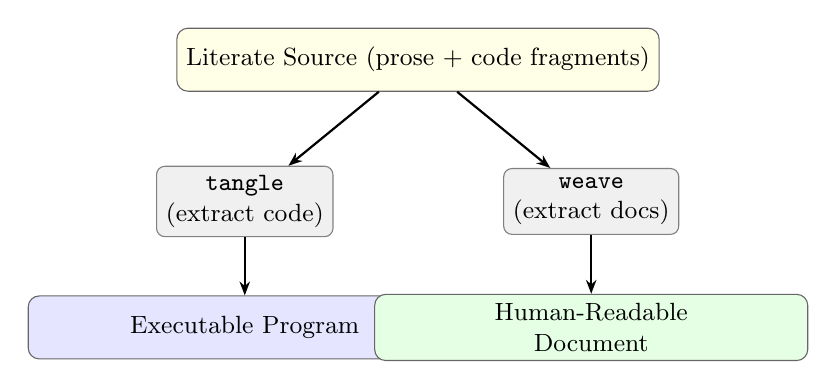
\begin{tikzpicture}[
  doc/.style={rectangle, draw=black!60, fill=yellow!10, rounded corners=4pt,
              minimum width=5.5cm, minimum height=0.8cm, font=\small, align=center},
  tool/.style={rectangle, draw=black!50, fill=gray!12, rounded corners=3pt,
               minimum width=2.2cm, minimum height=0.7cm, font=\small, align=center},
  arrow/.style={-{Stealth[length=5pt]}, thick}
]
  \node[doc] (src) at (0,0) {Literate Source (prose + code fragments)};

  \node[tool] (tangle) at (-2.2, -1.8) {\texttt{tangle}\\(extract code)};
  \node[tool] (weave)  at (2.2, -1.8)  {\texttt{weave}\\(extract docs)};

  \node[doc, fill=blue!10] (exe) at (-2.2, -3.4) {Executable Program};
  \node[doc, fill=green!10] (doc2) at (2.2, -3.4) {Human-Readable\\Document};

  \draw[arrow] (src) -- (tangle);
  \draw[arrow] (src) -- (weave);
  \draw[arrow] (tangle) -- (exe);
  \draw[arrow] (weave) -- (doc2);
\end{tikzpicture}
\caption{The literate programming toolchain \cite{knuth1984}. A single
source document containing interleaved prose and code fragments is
processed by two tools: \texttt{tangle} extracts executable code for
compilation, and \texttt{weave} formats the narrative for human reading.
The programmer's primary artifact is the explanation rather than the
program.}
\label{fig:literate}
\end{figure}

The resistance that literate programming has encountered within
mainstream technical culture is itself instructive. Most programmers
trained within conventional environments have internalized an interface
ecology in which the executable artifact is primary. Documentation is
experienced as overhead, a tax imposed on the act of computation rather
than its substance. The literate programming inversion therefore feels
cognitively unnatural to those whose motor language was formed within
systems that privilege execution over explanation \cite{brooks1975}.

This resistance illustrates the depth of the scope memeplex. Even a
practice that promises demonstrable benefits in code clarity and
maintainability can fail to achieve widespread adoption if it requires
practitioners to abandon the interaction grammar through which they have
organized their professional identity.

The tool becomes the measure of the thought it enables.

\section{Concurrency, Channels, and the Grammar of Parallel Processes}

The preceding analysis has focused primarily on sequential interaction
models. Yet modern computing increasingly requires reasoning about
processes that execute simultaneously, communicate asynchronously, and
may interfere with one another in subtle ways. The ecological
consequences of this shift deserve examination.

The formal study of concurrent processes has produced several distinct
computational models, each of which cultivates its own interaction
grammar and associated cognitive ecology. Hoare's Communicating
Sequential Processes (\textsf{CSP}) describes concurrency through the
synchronous rendezvous of independent processes \cite{hoare1985}. Two
processes communicate by simultaneously performing complementary input
and output actions on a named channel; neither can proceed until the
other is ready.

\begin{definition}[CSP Process Algebra]
In \textsf{CSP}, a process $P$ is defined by the grammar
\[
P \;::=\; \mathbf{STOP} \;\mid\; \mathbf{SKIP} \;\mid\; a \to P
        \;\mid\; P \,\Box\, Q \;\mid\; P \,\|\,\, Q
\]
where $a \to P$ denotes performing action $a$ then behaving as $P$;
$P \,\Box\, Q$ is an external choice between $P$ and $Q$; and
$P \,\|\,\, Q$ denotes the parallel composition of $P$ and $Q$ with
synchronized communication \cite{hoare1985}.
\end{definition}

The cognitive model cultivated by \textsf{CSP} is distinct from both
the sequential imperative model and the compositional Unix model. A
programmer working within \textsf{CSP} conceives of computation as a
collection of independent agents whose coordination emerges from the
structure of their communication topology. Individual process behavior
is secondary to the interaction protocol.

\begin{figure}[h]
\centering
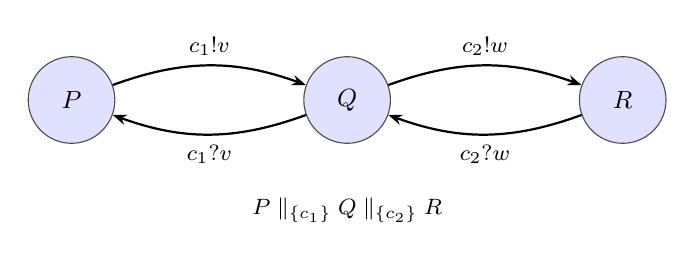
\begin{tikzpicture}[
  proc/.style={circle, draw=black!70, fill=blue!12, minimum size=1.1cm, font=\small},
  chan/.style={font=\footnotesize\itshape},
  arrow/.style={-{Stealth[length=5pt]}, thick, bend left=20}
]
  \node[proc] (A) at (0, 0)    {$P$};
  \node[proc] (B) at (3.5, 0)  {$Q$};
  \node[proc] (C) at (7, 0)    {$R$};

  % Channels
  \draw[arrow] (A) to node[above, chan]{$c_1 ! v$} (B);
  \draw[-{Stealth[length=5pt]}, thick, bend left=20] (B) to node[below, chan]{$c_1 ? v$} (A);
  \draw[arrow] (B) to node[above, chan]{$c_2 ! w$} (C);
  \draw[-{Stealth[length=5pt]}, thick, bend left=20] (C) to node[below, chan]{$c_2 ? w$} (B);

  \node[font=\footnotesize] at (3.5, -1.4)
    {$P \parallel_{\{c_1\}} Q \parallel_{\{c_2\}} R$};
\end{tikzpicture}
\caption{A \textsf{CSP} process network. Processes $P$, $Q$, $R$ run
concurrently and communicate via synchronous channel operations:
$c\,!\,v$ sends value $v$ on channel $c$; $c\,?\,v$ receives it.
Communication requires both parties to be simultaneously ready,
enforcing a rendezvous discipline \cite{hoare1985}.}
\label{fig:csp}
\end{figure}

The interaction grammar of concurrent programming environments
consequently diverges sharply from that of sequential ones. Where the
sequential programmer reasons about the transformation of state through
time, the concurrent programmer must reason about the interleaving of
multiple timelines and the communication protocols that bind them.

The scope memeplex of concurrency is correspondingly fragmented. Threads
and shared memory, channels and message passing, actors and mailboxes,
software transactional memory---each model cultivates a distinct
cognitive ecology, and the communities that form around them exhibit
familiar patterns of ideological commitment. Advocates of shared-memory
concurrency emphasize raw performance and direct access to machine
architecture. Channel-based systems encourage compositional protocol
reasoning. Actor systems promise fault isolation. Each group is partially
correct, because each model genuinely is better suited to certain classes
of problems.

Yet the theoretical equivalence between these models is often
overlooked in practice \cite{kleene1952}. Any sufficiently expressive
concurrent model can simulate any other, at the cost of additional
encoding overhead. The practical differences therefore lie not in
expressive power but in the cognitive ergonomics of reasoning about
concurrency under each model's particular grammar.

\section{Conclusion: Toward a Truce in the Tooling Wars}

The recurring conflicts that animate technical culture---editor wars,
keyboard wars, language wars, and the innumerable skirmishes over
frameworks and development environments---often present themselves as
arguments about technical correctness. Each community defends its
preferred tools with a mixture of practical reasoning, aesthetic
judgment, and occasionally missionary zeal.

Yet the deeper analysis offered by theoretical computer science suggests
a different interpretation.

The equivalence of the lambda calculus and the Turing machine
demonstrates that computational expressiveness is remarkably stable
across formal systems \cite{church1936,turing1936,kleene1952}. Any
paradigm that achieves computational universality can, in principle,
simulate any other. Functional, imperative, declarative, and
object-oriented approaches therefore differ not in the fundamental
problems they can solve but in the conceptual pathways they provide for
solving them \cite{backus1978}.

The same observation extends to interfaces and interaction models.
Command-line environments emphasize compositional transformation
\cite{ritchie1974,mcilroy1978}. Graphical systems emphasize spatial
manipulation. Modal editors encourage symbolic grammar through motor
memory, while integrated development environments present structured
visual representations of program state \cite{norman1988}.

Each approach offers a different cognitive coordinate system for
navigating the same computational terrain.

The intensity of the resulting debates can therefore be understood as a
consequence of the scope memeplex described throughout this essay.
Repeated interaction with a particular tool gradually reshapes both the
motor habits and conceptual metaphors of its users. Over time these
habits become intertwined with professional identity
\cite{norman1988,brooks1975}. A keyboard layout, an editor configuration,
or a scripting environment ceases to be merely instrumental and begins
to feel like the natural order of things.

From this perspective the tooling wars resemble linguistic disputes
between speakers of closely related dialects. Each group experiences its
own vocabulary and grammar as intuitive while regarding alternatives as
awkward or unnecessarily complicated.

The underlying computational substrate, however, remains unchanged.

Recognizing this fact does not require abandoning one's preferred tools.
On the contrary, deep familiarity with a well-chosen environment can
enable remarkable efficiency and creativity \cite{knuth1984}. What it
does suggest is a measure of intellectual humility. The elegance of a
particular workflow often reflects a fortunate alignment between a
tool's design and a user's cognitive style rather than the discovery of
a universal law of software engineering.

In this sense the great editor wars and keyboard schisms may ultimately
serve a useful cultural function. They reveal how strongly programmers
care about the instruments through which they think.

But once the theoretical equivalence of computational models is taken
seriously, the ideological stakes of these disputes begin to diminish.
The Vim user, the Emacs devotee, the shell traditionalist, and the
enthusiast of graphical environments are all exploring the same
computational universe from different vantage points \cite{raymond2003}.

The machines beneath their arguments continue to evaluate functions with
quiet impartiality.

And somewhere in the background, small composable programs still wait to
be connected by pipes.

\newpage
\begin{thebibliography}{99}

\bibitem{church1936}
Alonzo Church.
\newblock An Unsolvable Problem of Elementary Number Theory.
\newblock \emph{American Journal of Mathematics}, 58(2):345--363, 1936.

\bibitem{turing1936}
Alan M. Turing.
\newblock On Computable Numbers, with an Application to the Entscheidungsproblem.
\newblock \emph{Proceedings of the London Mathematical Society}, 42:230--265,
  1936.

\bibitem{kleene1952}
Stephen C. Kleene.
\newblock \emph{Introduction to Metamathematics}.
\newblock North-Holland, 1952.

\bibitem{fant2006}
Karl J. Fant.
\newblock \emph{Computer Science Reconsidered: The Invocation Model of Process
  Expression}.
\newblock Wiley-Interscience, 2006.

\bibitem{kernighan1978}
Brian W. Kernighan and Dennis M. Ritchie.
\newblock \emph{The C Programming Language}.
\newblock Prentice Hall, 1978.

\bibitem{ritchie1974}
Dennis M. Ritchie and Ken Thompson.
\newblock The UNIX Time-Sharing System.
\newblock \emph{Communications of the ACM}, 17(7):365--375, 1974.

\bibitem{raymond2003}
Eric S. Raymond.
\newblock \emph{The Art of Unix Programming}.
\newblock Addison-Wesley, 2003.

\bibitem{mcilroy1978}
M. Douglas McIlroy.
\newblock Mass Produced Software Components.
\newblock In \emph{Proceedings of the NATO Conference on Software Engineering},
  1968.

\bibitem{hoare1985}
C.\ A.\ R. Hoare.
\newblock \emph{Communicating Sequential Processes}.
\newblock Prentice Hall, 1985.

\bibitem{backus1978}
John Backus.
\newblock Can Programming Be Liberated from the von Neumann Style?
\newblock \emph{Communications of the ACM}, 21(8):613--641, 1978.

\bibitem{brooks1975}
Frederick P. Brooks.
\newblock \emph{The Mythical Man-Month}.
\newblock Addison-Wesley, 1975.

\bibitem{norman1988}
Donald A. Norman.
\newblock \emph{The Design of Everyday Things}.
\newblock Basic Books, 1988.

\bibitem{yamada1980}
Hiroshi Yamada.
\newblock A Historical Study of Typewriter Keyboard Layouts.
\newblock \emph{IEEE Annals of the History of Computing}, 2(2):175--191, 1980.

\bibitem{stallman2002}
Richard M. Stallman.
\newblock \emph{Free Software, Free Society}.
\newblock GNU Press, 2002.

\bibitem{knuth1984}
Donald E. Knuth.
\newblock Literate Programming.
\newblock \emph{The Computer Journal}, 27(2):97--111, 1984.

\bibitem{barendregt1984}
Henk P. Barendregt.
\newblock \emph{The Lambda Calculus: Its Syntax and Semantics}.
\newblock North-Holland, revised edition, 1984.

\bibitem{pierce2002}
Benjamin C. Pierce.
\newblock \emph{Types and Programming Languages}.
\newblock MIT Press, 2002.

\bibitem{milner1999}
Robin Milner.
\newblock \emph{Communicating and Mobile Systems: The $\pi$-Calculus}.
\newblock Cambridge University Press, 1999.

\bibitem{wadler1992}
Philip Wadler.
\newblock The Essence of Functional Programming.
\newblock In \emph{Proceedings of the 19th ACM Symposium on Principles of
  Programming Languages}, pages 1--14, 1992.

\bibitem{floyd1979}
Robert W. Floyd.
\newblock The Paradigms of Programming.
\newblock \emph{Communications of the ACM}, 22(8):455--460, 1979.

\end{thebibliography}

\end{document}
